\chapter{Concept}
\section{Motivation}



\section{Architecture}

\begin{figure}
  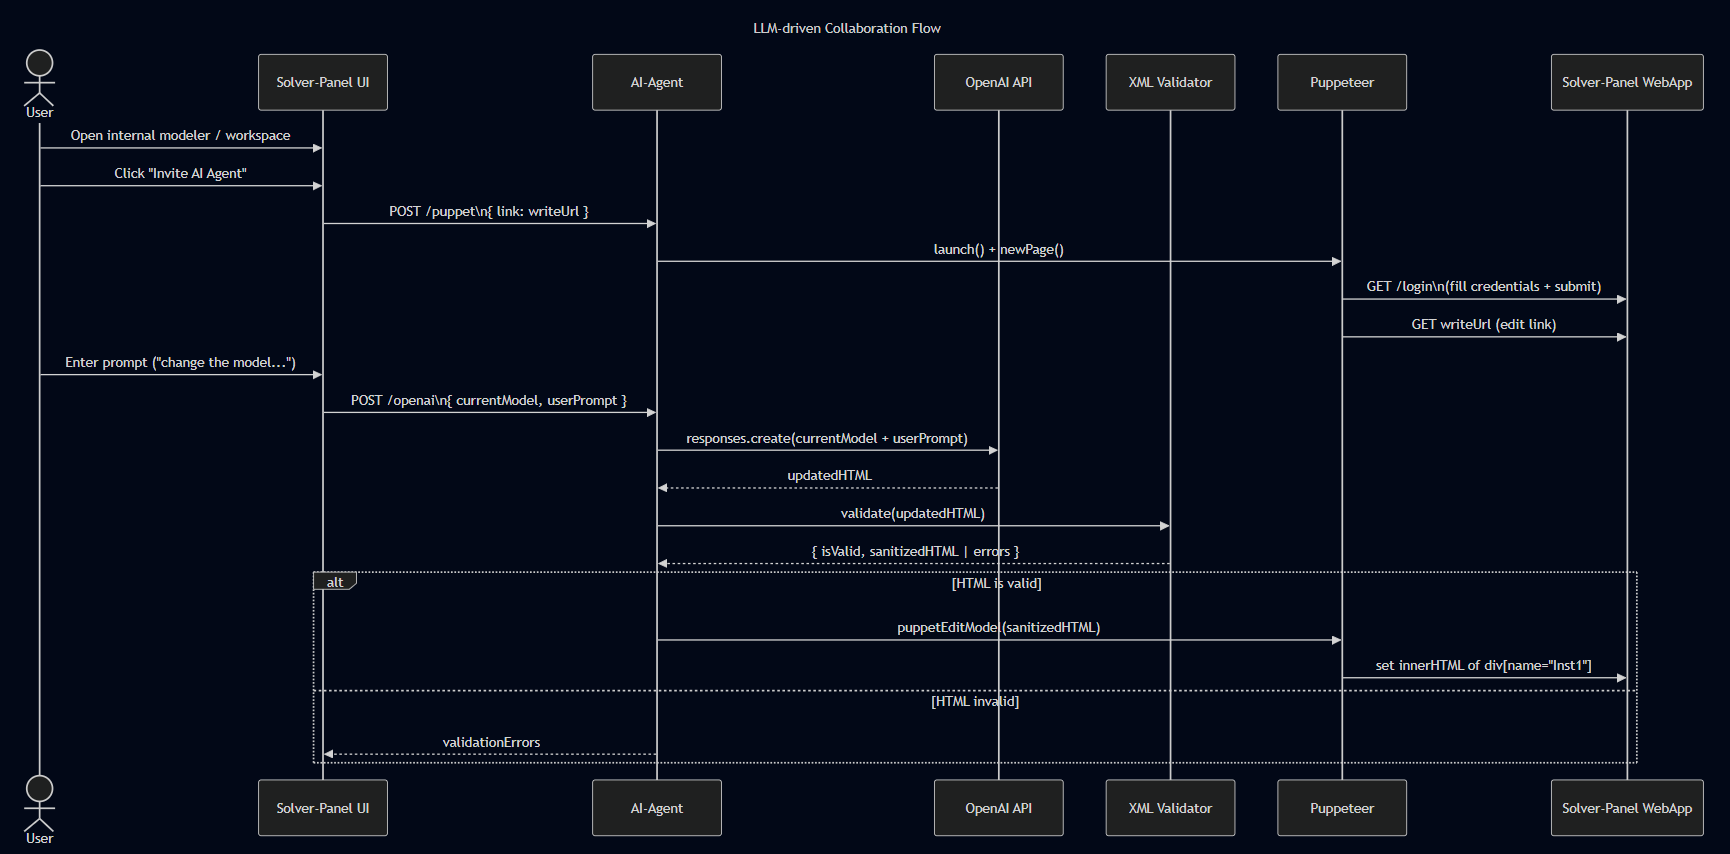
\includegraphics[width=\linewidth]{static/diagram_image.png}
  \caption{Sequence Diagram of the Architecture}
  \label{fig:sequence}
\end{figure}
Now lets get into the theoretical details of the architecture and see how everything actually comes together. The architecture can also be seen in \ref{fig:sequence}.

\begin{enumerate}
    \item \textbf{Node.js: } Node.js is a server-side framework for JavaScript which gives us the possiblity to run javascript code on the server. 
    \item \textbf{Environment for AI-Agent: } If we want the AI-Agent to join as a first-class collaborator in the optimization platform, the AI-Agent must have its own instance of modeler opened on a web-browser which it should also be able to access. 
    \item \textbf{Collaboration Mechanism: } The master user \cite{MarkoThesisMsc} registers and logs into the optimization platform hosted at \url{https://optimized.mpi-inf.mpg.de/modeler/} and initiates a new collaborative session. To start a collaborative session, the user must click on the \emph{Share} button located at the bottom of the interface, which opens a dialog containing shareable links for the workspace. Two links are provided in this dialog: an \textbf{edit link} and a \textbf{read link}. If another user is intended to join the workspace with editing privileges, the edit link should be shared; otherwise, the read link can be shared for view-only access. 

When the invited user clicks on the shared link, they can view the modeler instance and join the workspace as a collaborator. This explanation is necessary for the discussion that follows. User can also invite an AI-agent by clicking on the button called \emph{Invite AI-Agent}.

    \item \textbf{Invite AI-Agent : } Now lets see what does the \emph{Invite AI-Agent} button actually do and how its implemented. So as we know about the two types of links, clicking on them opens an instance of the shared modeler in the browser, 

    \item \textbf{Puppeteer : } It is the key component of the system. Puppeteer \cite{pptrPuppeteerPuppeteer} is a JavaScript framework that enables backend control of a Chromium \cite{chromiumHome}-based browser (Chrome, in our case) via browser automation APIs. This makes it possible to launch and control an instance of Chrome programmatically from the backend according to application requirements. 
    
    In our setup, an instance of Chrome is launched on the backend, and the framework’s APIs are used to navigate to the optimization platform’s web application, authenticate as the AI agent, and interact with the page by accessing and manipulating the DOM \cite{mozillaDocumentObject}. This allows the AI agent to apply changes directly to the web-based optimization model. A detailed explanation of this process is provided later in the architecture section.

    \item \textbf{Large Language Model : } This component represents the core of the architecture. A large language model (LLM) \cite{wikipediaLargeLanguage} is a type of language model that predicts the next token based on a probability distribution learned during training on large-scale datasets. Since the emergence of the Transformer architecture \cite{vaswani2023attentionneed}, language models have become significantly more powerful and expressive. As a result, they can now be effectively leveraged to generate and modify optimization models in response to high-level user requirements.

    \item \textbf{Validation : }

    \item \textbf{LangGraph : } This layer enables users to review the output generated by the LLM. LangGraph \cite{langchainLangGraph} is a JavaScript framework designed for constructing cyclic and stateful AI-agent workflows. In our implementation, once the AI model generates an output, the user is given the option to accept the result, reject it, or provide feedback. If the user chooses to provide feedback, the model regenerates the output by incorporating the feedback and presents the updated result to the user. This process forms an iterative cycle that continues until the user is satisfied with the outcome.
\end{enumerate}

\section{Design Decisions}